\section{Implementing Pegged Ledgers}
\label{sec:construction}

\todo{Clean up this section}

We present a construction for pegged ledgers
%over a generic epoch-based PoS blockchain
that is based
on Ouroboros PoS~\cite{ouroboros}, but also applicable to other PoS
systems such as Snow White~\cite{snowwhite}
and Algorand~\cite{algorand}.
Our protocol
will implement a system of ledgers with pegging %correctness and
security
according to
%Definition~\ref{def:correctness} and
Definition~\ref{def:security} under an assumption on the relative stake power of the
adversary that will be detailed below.

The main challenge in implementing pegged ledgers is to facilitate secure
cross-chain transfers.  We consider two approaches to such transfers and refer
to them as {\em direct observation} or {\em cross-chain certification}. Consider
two pegged ledgers $\Ledger_1$ and $\Ledger_2$.  Direct observation of $\Ledger_1$ means that
every node of $\Ledger_2$ follows and validates $\Ledger_1$; it is easy to see that this
enables transfers from $\Ledger_1$ to $\Ledger_2$.  On the other hand, cross-chain
certification of $\Ledger_2$ means that $\Ledger_1$ contains appropriate cryptographic
information sufficient to validate data issued by the nodes following $\Ledger_2$.
This allows transfers of assets from $\Ledger_2$, as long as they are certified, to be
accepted by $\Ledger_1$-nodes without following $\Ledger_2$.
The choice between direct observation and cross-chain certification can be made
independently for each direction of transfers between $\Ledger_1$ and $\Ledger_2$, any of
the 4 variants is possible (cf. Figure~\ref{fig:sidechain-options}).

Another aspect of implementing pegged ledgers in the PoS context is the choice
of stake distribution that underlies the PoS on each of the chains.
We again consider two options, which we call  {\em independent
staking} and {\em merged staking}. In independent staking, blocks on
say $\Ledger_1$ are ``produced by'' coins from $\Ledger_1$ (in other words, the
block-creating rights on $\Ledger_1$ are attributed based on the stake distribution
recorded on $\Ledger_1$ only).
In contrast, with merged staking, blocks on $\Ledger_1$ are
produced either by coins on $\Ledger_1$, or coins on $\Ledger_2$ that have, via their
staking key, declared support of $\Ledger_1$ (but otherwise remain on $\Ledger_1$); see
Figure~\ref{fig:sidechain-options}. Also here, all 4 combinations are possible.

\begin{figure*}
\begin{center}
    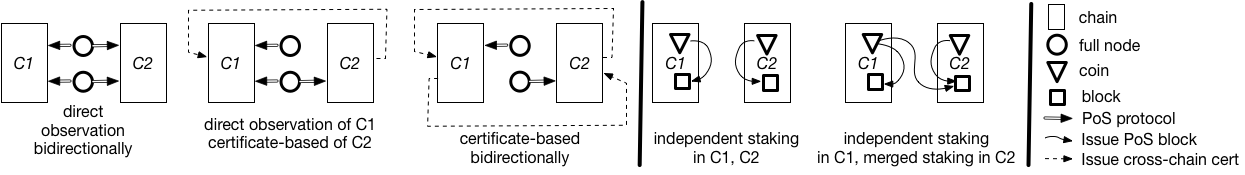
\includegraphics[width=\textwidth]{chapters/sidechains/figures/sidechains-options.png}
  \caption{Deployment options for PoS Sidechains.}
  \label{fig:sidechain-options}
  \end{center}
\end{figure*}

In our construction we choose an exemplary
configuration between two ledgers $\Ledger_1$ and
$\Ledger_2$, so that direct observation is applied to $\Ledger_1$,
cross-chain certification to $\Ledger_2$, independent-staking in $\Ledger_1$ and
merged staking in $\Ledger_2$.
As a result, all stakeholders in $\Ledger_2$ also keep track
of chain development on $\Ledger_1$ (and hence run a full node for $\Ledger_1$)
while the opposite is not necessary, i.e.,
$\Ledger_1$ stakeholders can be oblivious of transactions and
blocks being added to $\Ledger_2$.
This illustrates the two basic possibilities
of pegging and can be easily adapted
to  any other of the configurations between two ledgers in Figure~\ref{fig:sidechain-options}.

In order to reflect the asymmetry between the two chains in our exemplary
construction we will refer to $\Ledger_1$ as the ``mainchain'' $\Mainchain$, and to
$\Ledger_2$ as the ``sidechain'' $\Sidechain$. To elaborate further on this concrete
asymmetric use case, we also fully specify how the sidechain can be
initialized from scratch, assuming that the mainchain already exists.


%We also assume (as discussed in Section~\ref{sec:model}) that all
%actors have relatively synchronized clocks: i.e., clock drift is bounded
%and time can be divided in time slots that all parties can agree on.
%During the existence of the mainchain $\Mainchain$,
%the sidechain can come to existence whenever a new epoch starts on $\Mainchain$.

The pegging with the sidechain will be provided with respect to a specific asset of $\Mainchain$
that will be created on $\Mainchain$.
% PG: not used ever again
%and referred to as the \emph{home} asset of the
%whole sidechain ecosystem.
Note that $\Mainchain$ as well as $\Sidechain$ may carry
additional assets but for simplicity we will assume that staking and pegging is
accomplished only via this single primary asset.

The presentation of the construction is organized as follows. First, in Section~\ref{sec:ats} we introduce a novel
cryptographic primitive, \emph{ad-hoc threshold multisignature (ATMS)}, which is the fundamental building block for cross-chain certification.
Afterwards, in Section~\ref{sec:const} we use it as a black box to build secure
pegged ledgers with respect to concrete instantiations of the functions $\merge$
and $\effect$ and a validity language $\adalang$ for asset~$\ada$ given in Section~\ref{sec:inst}.
Finally, we discuss specific instantiations of ATMS in
Section~\ref{sec:auth}.


\import{chapters/sidechains/}{tms-definition.tex}
\import{chapters/sidechains/}{adalang.tex}

\subsection{The Sidechain Construction}
\label{sec:const}

We now describe the procedures for running a sidechain in the configuration
outlined at the beginning of this section: with independent staking on $\MC$ and
merged staking on $\SC$; direct observation of $\MC$ and
cross-chain certification of $\SC$.
We describe the sidechain's creation,
maintenance, and the way assets can be  transferred to it and back.  The
protocol we describe below is quite complex,
%(it entails 2 consensus protocols
%for maintaining both the mainchain and the sidechain, and a lot of connecting
%tissue)
%and to accommodate that, while still keeping the protocol description at
%a manageable length,
we hence choose to describe different parts of the protocol in
differing levels of detail. This level is always chosen with the intention to allow the
reader to easily fill in the details.
%, and to follow our security argument in Section~\ref{sec:security}.
A graphical depiction of our construction that can serve as a reference
%for the reader of the description below
is given in Figure~\ref{fig:sidechain}.
\begin{figure}[tb]%{{{
  \centering
  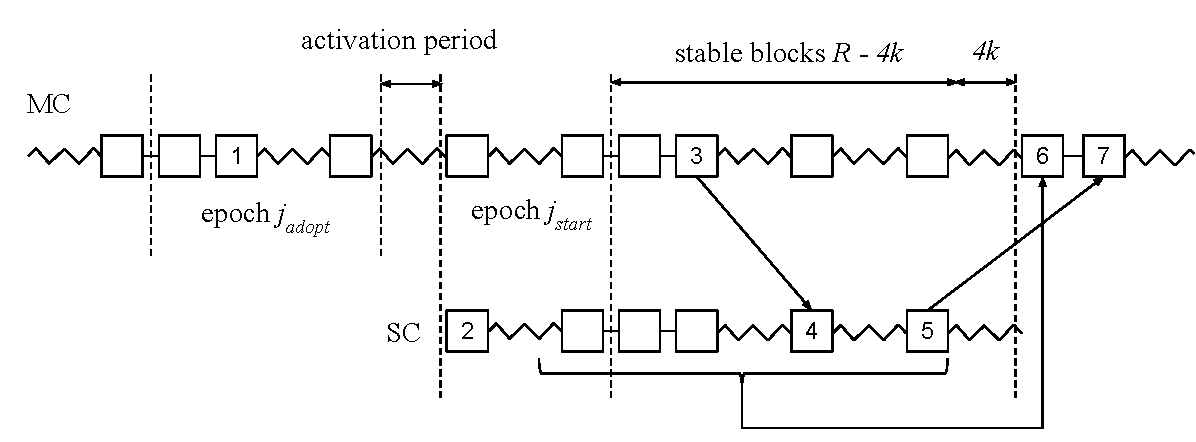
\includegraphics[width=0.8\textwidth]{chapters/sidechains/figures/sidechains-overview.pdf}
  \caption{
  Our sidechain construction. Blocks are shown as rectangles. Adjacent blocks
  connect with straight lines. Squiggly lines indicate some blocks are omitted.
  $\MC$ is at the top, $\SC$ at the bottom. Epochs are separated by dashed
  lines. $\epoch_{j_\text{adopt}}$ is the epoch of first signalling;
  $\epoch_{j_\text{start}}$ is the activation epoch. Blocks of interest: 1. The
  first block signalling $\SC$ awareness;
  2. The $\SC$ genesis block; 3. A $\tx_{\send}$
  transaction for a deposit; 4. A $\tx_{\rec}$ transaction for a
  deposit; 5. A $\tx_{\send}$ transaction for withdrawal; 6. A $\sccert$
  transaction signalling trust transition within $\SC$ and certifying pending
  withdrawals; 7. A $\tx_{\rec}$ transaction for withdrawal, certified in a $\sccert$
  transaction e.g. in block~6.
  }
  \label{fig:sidechain}
\end{figure}%}}}

\subsubsection{Notation}
Where applicable, we denote the analogues of the mainchain objects on the
sidechain with an additional overline.
%For instance, while $\SD_j$ denotes the
%stake distribution recorded on the mainchain by the latest block in
%the first $4k$ slots of epoch $j-1$ (which is the stake distribution used for
%sampling slot leaders for epoch $j$ on $\MC$), $\SDb_j$ will denote
%the stake distribution induced by the stake that resides on $\SC$ at the same
%slot (this would be the stake distribution used for sampling slot leaders for
%epoch $j$ if $\SC$ was using independent staking).
%Finally, we let  $\SDb^*_j$ denote  the distribution of stake
%that exists in either the sidechain or the mainchain, but has indicated
%sidechain adoption (as discussed below) by the end of the first $4k$ slots of epoch $\epoch_{j-1}$.
%This will be the stake
%distribution \emph{actually used} for leader election on $\SC$ in epoch $j$ as
%per the merged staking paradigm.
%
In our pseudocode, we use the statement
``\textbf{post} $\tx$ \textbf{to} $\Ledger$''
to refer to the
action of broadcasting the transaction $\tx$ to the maintainers of the ledger
$\Ledger$ so that they include it in the ledger eventually as prescribed by the
protocol.
Unless indicated otherwise, we also denote by $\stateMC$ (resp.
$\stateSC$) the current \emph{ledger state} of the ledger $\MC$ (resp. $\SC$) as
viewed by the party executing the protocol. Similarly, we denote by $\ChainMC$
(resp. $\ChainSC$) the currently held \emph{chain} corresponding to the ledger
$\MC$ (resp. $\SC$). Hence, for example $\stateMC$ always represents the state
stored in the stable part of the chain $\ChainMC$.

\subsubsection{Helper Transactions and Data}
The construction uses a set of \textit{helper transactions}
which can be included in both blockchains, but do not get reported
in the respective ledgers. These helper transactions store the appropriate
metadata which is implementation-specific and allow the pegging functionality to be
maintained. The transaction types $\mathsf{side}\-\mathsf{chain\_support}$,
$\mathsf{side}\-\mathsf{chain\_certificate}$,
$\mathsf{side}\-\mathsf{chain\_success}$ and
$\mathsf{side}\-\mathsf{chain\_fai}\-\mathsf{lure}$, whose nature will be
detailed later, are of this kind.
Moreover, our concrete implementation of pegged ledgers extends certain
transactions with additional information (such as Merkle-tree inclusion proofs)
that are, for convenience, understood to be stripped off these transactions when
the blockchain is interpreted as a ledger.

\subsubsection{Initialisation}

The creation of a new sidechain~$\SC$ starts by any of the stakeholders of the
mainchain adopting the code that implements the sidechain. This action does not
require the stakeholders to put stake on the sidechain but merely to run the
code to support it (e.g. by installing a pluggable module into their client
software). In the following this is referred to as ``adopting the sidechain''
and captured by the predicate $\SidechainAdoption$.
The adoption is  announced at the mainchain by a special transaction
detailed below.  Each sidechain is identified by a unique identifier $\id_\SC$.
%The identifier is a simple string,
%which must be chosen to be unique for that particular sidechain,
%. For example,
%the first attempt at launching a smart-contract-supporting sidechain could have
%the identifier
%e.g. ``\texttt{computation\_layer\_1.0.0}''. As mentioned, we consider a
%single sidechain which we will refer to as $\SC$, but our results extend to
%multiple sidechains sharing the same mainchain.

Let $\jadopt$ denote the epoch on $\MC$ when the first adoption transaction has
appeared; the sidechain $\SC$ -- if its activation succeeds as discussed
below -- will start at the beginning of some later epoch $\jstart$ and will have
its slots and epochs synchronized with $\MC$.
The software module implementing the sidechain comes with a set of
deterministic rules describing the requirements for the successful activation of
the sidechain, as well as for determining $\jstart$.
These rules are sidechain-specific and are captured in a predicate
$\ActSuccess$ and a function $\ActEpoch$, respectively.
One typical such example is the following:
the sidechain starts at the beginning of $\MC$-epoch $\jstart$ for the smallest
$\jstart$ that satisfies:
%\begin{itemize}
  %\item
    (i)  $\jstart - \jadopt > c_1$;
  %\item
    (ii) at least $c_2$-fraction of stake on $\MC$ is controlled by stakeholders that
    have adopted $\SC$;
%\end{itemize}
for some constants $c_1$,$c_2$. Additionally, if such a successful activation
does not occur until a failure condition captured by a predicate
$\ActFail$ is met (e.g. until a predetermined period of $c_3>c_1$ epochs has
passed), the sidechain initialization is aborted.
%The exact mechanics of the abortion procedure are also left to be
%determined by the sidechain module (we denote them as $\SC.\Cleanup()$)
%but they include straightforward actions such
%as removing the module that supports the sidechain and erasing any other data
%structure associated with it.
%\footnote{We note that there is nothing that
%prevents a minority of $\MC$ stakeholders from continuing to support an aborted
%sidechain if they insist, in violation of the sidechain creation rules. However
%all the other stakeholders of $\MC$ will consider the sidechain as failed, and
%assuming they represent the majority of stake, any blocks produced by the
%diverging stakeholders that reference the failed sidechain will be collectively
%removed from the ledger of $\MC$. On the other hand, if the majority of stake in
%$\MC$ insists on the violation of the sidechain creation rules, we observe that
%the constants $c_1,c_2$ can be effectively changed by a soft-fork of $\MC$. Such
%soft-forks can be avoided by choosing relatively low values for $c_1,c_2$. On
%the other hand, it is important to note that really low values for $c_1,c_2$ may
%result in unnecessarily cluttering the $\MC$ with data related to sidechains
%that are spuriously created. }

%%Suppose the first occurrence of sidechain adoption is
%%announced by a stakeholder at epoch $j^*$ of $\MC$ for some $j^* \geq 2$. Then the
%%sidechain will be created at epoch $\epoch_j$ for some $j > j^*$. The sidechain
%%genesis block is created at the first slot of epoch $\epoch_j$.

%The way $j$ is determined based on $j^*$ is as follows. Each sidechain defines
%an \textit{activation predicate} $\on^{\ell_1, \ell_2, \ell_3}(\Chain[:-k])$,
%parameterized by integers $\ell_1, \ell_2, \ell_3 \in \N$, which is evaluated on
%the stable part $\Chain[:-k]$ of some chain $\Chain$. At every slot after epoch
%$j^*$, the honest stakeholders on the network evaluate the predicate $\on$ on the
%growing stable part of the mainchain $\Chain[:-k]$, where $\Chain$ is their
%currently locally adopted mainchain.

%The predicate $\on^{\ell_1, \ell_2, \ell_3}(\Chain)$ checks that all of the following conditions are
%satisfied:
%\begin{enumerate}
%    \item The chain length is sufficient: $|\Chain| > \ell_1$.
%    \item Sufficient stake has been moved into limbo: $|\SDb| > \ell_2$
%          (the exact definition of stake movement will follow momentarily).
%    \item Sufficient stake is aware of the sidechain: $|\SDb^*| > \ell_3$
%          (the exact definition of stake awareness will follow momentarily).
%    \item There is a sufficient epoch gap:
%          If the first adoption announcement occurred after or at slot
%          %$R - 2k/f$
%          $R - 2k$
%          of epoch $\epoch_{j^*}$, the current slot must belong to $\epoch_j$, with
%          $j > j^*$.
%\end{enumerate}
%The sidechain is considered activated during the first slot at which its
%$\on^{\ell_1, \ell_2, \ell_3}$
%predicate is evaluated to \textit{true}. The genesis block $\Genesisb$ of the
%sidechain is then created at the first slot of the first epoch after the slot
%during which the sidechain was activated.

%Each sidechain also defines an \textit{expiration predicate}
%$\off^{\ell_4}(\Chain[:-k])$, parameterized by $\ell_4 \in \N$, which is also
%evaluated on the stable part of the mainchain. As long as the sidechain has not
%yet been activated, at every slot after epoch $j^*$, each honest maintainer
%evaluates the predicate $\off$ on the growing stable part of the mainchain
%$\Chain[:-k]$, where $\Chain$ is their currently locally adopted mainchain. The
%predicate $\off$ checks whether the chain length is too large: $|\Chain| >
%\ell_4$.
%If at some slot the predicate $\off(\Chain)$ evaluates to \textit{true} while at
%the same slot the predicate $\on(\Chain)$ evaluates to \textit{false}, then the
%sidechain creation is abandoned and we say that the sidechain creation has
%\textit{expired}. No sidechain genesis block $\Genesisb$ is created. Of course,
%for meaningful sidechains, we have that $\ell_4 > \ell_1$ to give the sidechain
%a period of time during which it can be created. If a sidechain's creation
%expires, then it will never be created. An attempt can be made in the future to
%create a new sidechain with the same features, but with a new identifier.

%During the period after the first awareness announcement block and before the
%sidechain is created or expires, we allow stake to be moved from the mainchain
%to the sidechain. The mechanics for the stake transfers is described later in
%this section. For now, suppose there is a way to move money out of the mainchain
%via a $\mathsf{sidechain\_send}$ transaction which is included in a mainchain
%block. As the sidechain has not yet been created, this money is kept in
%\textit{limbo} in that it has been moved out of the mainchain but not yet into
%the sidechain, in the sense that it cannot yet be recovered. If the sidechain is
%successfully created at epoch $\epoch_j$, then the money in limbo that was moved
%from the mainchain into the sidechain during the period after the first
%awareness announcement and until the first activation can be recovered into the
%sidechain. This recovery can happen during the sidechain genesis block or at
%later blocks. However, if the sidechain creation expires, then the money in
%limbo can be returned to its previous owners on the mainchain by issuing dual
%reverting transaction, $\mathsf{sidechain\_recover}$, and including it on the
%mainchain.

The activation process then follows the steps outlined below, the detailed
description is  given in
%Appendix~\ref{sec:algorithms} as
Algorithm~\ref{alg.init}).
\import{chapters/sidechains/}{algorithms/alg.sc-init}
%\begin{enumerate}
%\item
    First, every stakeholder $U_i$ of $\MC$ (holding a key pair $(vk,sk)$) that supports the sidechain
    posts a special transaction
    $
    \mathsf{sidechain\_support}(\id_\SC,vk,vk')
    $,
    signed by $sk$
    into the mainchain. Here $vk'$ is a public key from an ATMS key pair
    freshly generated by $U_i$; its role is explained in Section~\ref{sec:trust}
    below.
    %at blocks created after epoch $j^*$.
    %, where
    %the initial adoption stakeholder distribution $\SDb^*_{j^*}$ of the
    %sidechain is initially empty.

  %\item
    If the sidechain activation succeeds, then during the first slot of epoch $\jstart$
    the stakeholders of $\MC$ that support $\SC$  construct the genesis block
    $
    \Genesisb
    =(
      \id_\SC,
      \SDb_{\jstart},
      \rndb_{\jstart}\defeq H( \id_\SC, \rnd_{\jstart}),
      \params,
      avk^{\jstart}
    )
    $
    for $\SC$. $\rnd_{\jstart}$ is the
    randomness for leader election on $\MC$ in epoch $\jstart$ (derived
    on $\MC$ in epoch $\jstart-1$). It is reused to compute the
    initial sidechain randomness
    $\rndb_{\jstart}$ as well, further
    $\rndb_{j'}$ for $j'>\jstart$ are determined independently on $\SC$ using
    the Ouroboros coin-tossing protocol.\footnote{This can be interpreted as
    using $\MC$ to implement the setup functionality needed to bootstrap $\SC$.
    }
    Furthermore, $\params$ and $avk^{\jstart}$ are public parameters and an aggregated public
    key of an ATMS scheme; their creation and role is
    discussed in Section~\ref{sec:trust} below.
    Note that $\Genesisb$ is defined mostly for notational compatibility, as
    $\SDb_{\jstart}$ is empty at this point anyway.
    %Note that this requires
    %$j\geq j^*+2$, as $\SDb_{j'}$ for $j'<j+2$ are empty. This can be enforced
    %as a part of the $\on$ predicate.
    $\Genesisb$ can be constructed as soon as %both $\SDb_{\jstart}$ and
    $\rnd_{\jstart}$ is known and stable.
    %, which is true as soon as the mainchain is stable up to
    %slot $16k/f$ of epoch ${j-1}$.

  %\item
    The stakeholders that adopted $\SC$ post into $\MC$
    %in the first block of epoch $\epoch_j$
    a transaction $\mathsf{sidechain\_success}(\id_\SC)$ to
    signify that $\SC$ has been initialized.
    If the sidechain creation expires, then, after the first block of the next
    epoch after expiration occurs, the stakeholders of $\MC$ that supported
    $\SC$ post the transaction $\mathsf{sidechain\_failure}(\id_\SC)$ to $\MC$.
    We assume that both predicates $\ActSuccess$ and $\ActFail$ can be evaluated
    based on the state of $\MC$ only, and hence spurious success/failure
    transactions will be considered invalid.
    %Upon
    %posting this message, refund transactions can be issued on the mainchain.

%\end{enumerate}

%Note that as soon as a sidechain is created it holds that an initial
%stakeholder distribution for the sidechain is known by the maintainers of the
%ledger state of $\MC$. We will maintain this property: the $\MC$ ledger state
%will always have a relatively current commitment to the stakeholder distribution
%of $\SC$.

%\newpage

\subsubsection{Maintenance}

Once the sidechain is created, both the mainchain and the sidechain need to be
maintained by their respective set of stakeholders (detailed below) running
their respective instance of the Ouroboros protocol.
%. In both
%cases this is done by running a slightly modified version of the Ouroboros
%protocol as follows.

In the case of the mainchain, the maintenance procedure is given
in Algorithm~\ref{alg.maintain.MC}.
This algorithm is run by all stakeholders controlling stake that is recorded on
the mainchain. Each stakeholder, on every new slot, collects all the candidate
$\MC$-chains from the network (modelled via the $\Diffuse$ functionality) and
filters them for both consensus-level validity (using $\MC.\ValidConsLevel$) and
transaction validity (using the $\verifierMC$ predicate given in
Algorithms~\ref{alg.mainchain} and~\ref{alg.mainchain-tx}). Out of the remaining valid chains, he chooses
his new state $\Chain_{\MC}$ via $\PickWinningChain$. Then the stakeholder
evaluates whether he is an eligible leader for this slot, basing its selection
on the stake distribution $\SD_j$ and randomness $\rnd_j$, which are determined
once per epoch
%in the $\SwitchMCEpoch$ function
in accordance with the Ouroboros protocol.
If the stakeholder finds out he is a slot leader, he creates a new block $B$ by
including all transactions currently valid with respect to $\Chain_{\MC}$
(as per the predicate $\verifierMCtx$ given also in Algorithm~\ref{alg.mainchain-tx}),
appends it to the chain $\Chain_{\MC}$ and diffuses the result\footnote{
As in~\cite{C:KRDO17,EC:DGKR18}, we simplify our
presentation by diffusing the complete chains,
although a practical implementation would only diffuse the block $B$.}
for other parties to adopt.

\import{chapters/sidechains/}{algorithms/alg.mc-maintain.tex}
\import{chapters/sidechains/}{algorithms/alg.mainchain.tex}

The maintenance procedure for $\SC$ is similar, hence we only
describe here how it differs from Algorithm~\ref{alg.maintain.MC}. Most
importantly, it is executed by all stakeholders who have adopted $\SC$,
irrespectively of whether they own any stake on $\SC$.
Recall that the slots and epochs of the $\SC$-instance of Ouroboros are aligned
with the slots and epochs of $\MC$.

The first difference is that all ocurrences of $\MC$ and $\ChainMC$ are
naturally replaced by $\SC$ and $\ChainSC$, respectively.  This also means that
the validity of received chains (resp. transactions), determined on
line~\ref{line:filter} (resp.~\ref{line:filtertx}), is decided based on
predicate
$\verifierSC(\cdot,\ChainMC)$ (resp.
$\verifierSCtx(\cdot)$)
instead of
the predicate
$\verifierMC(\cdot)$ (resp.
$\verifierMCtx(\cdot)$). Additionally, note that $\verifierSCtx$ must be called
with a sequence of transactions containing both the transactions in $\SC$ as
well as the transactions in $\MC$ interspersed and timestamped, similarly to the
way done in Line~\ref{alg.sidechain.interspersing} of
Algorithm~\ref{alg.sidechain}. This is straightforward to implement, as the
sidechain maintainers also directly observe the mainchain. The predicates
$\verifierSCtx$
and
$\verifierSC$
are given in
Algorithms~\ref{alg.sidechain-tx}
and~\ref{alg.sidechain}, respectively.

\import{chapters/sidechains/}{algorithms/alg.sidechain-figure.tex}

Second, instead of the
%the procedure $\SwitchMCEpoch$ on
%line~\ref{line:switch} is replaced by the procedure $\SwitchSCEpoch$ (given in
%Algorithm~\ref{alg.maintain.SC}) that determines a different
stake distribution $\SD_j$ determined on line~\ref{line:SD}, a different
distribution $\SDb^*_j$ is determined to be used for slot leader selection in
the $j$-th epoch of the sidechain.  The distribution $\SDb^*$ contains all
stake belonging to stakeholders that have adopted $\SC$, irrespectively of
whether this stake is located on $\MC$ or $\SC$ (we call such stake
\emph{$\SC$-aware}).  It can be obtained by combining the distribution $\SDb$ as
recorded in $\SC$ with the distribution of $\SC$-aware stake on $\MC$ (which is
known to $\SC$-maintainers via direct observation of $\MC$).
%This is
%in contrast to a hypothetical stand-alone execution of Ouroboros  on $\SC$,
%which would only use the stake distribution $\SDb$ instead.
Note that the
distribution used for epoch $j$ reflects the stake distribution of $\SC$-aware
stake in the past, namely by slot $4k$ of epoch $j-1$, just as in $\MC$.
%The randomness $\rndb_{j}$ for each epoch $j$
%is derived deterministically from the mainchain randomness for the same
%epoch $\rnd_j$, concretely $\rndb_{j}\defeq H(\id_\SC, \rnd_{j})$.
%This is done for efficiency reasons as the randomness in Ouroboros is
%derived via a relatively costly coin-tossing protocol, and its reuse on the
%sidechain does not harm security.
Naturally, this also implies that the fourth parameter for the $\SlotLeader$ predicate on
line~\ref{line:leader} is  $\SDb^*_j$ %and $\rndb_j$
instead of $\SD_j$.
% and $\rnd_j$, respectively.

Finally, the block construction procedure on line~\ref{line:construct} is
adjusted so that in the last $2k$ slots of each epoch, the created blocks on the
sidechain also
contain an additional ATMS signature of a so-called sidechain certificate (how
this certificate is constructed and used will be described below). Hence,
whenever $\slot\mod R>10k$, line~\ref{line:construct} is replaced by
$
  B
  \leftarrow
  (\prev,\vec\tx_{\valid},\sigma,\sigma_{\sccert_{j+1}})
$
where
$\sigma_{\sccert_{j+1}}=\Sig_{sk}(\sccert_{j+1})$ and $j$ is the current epoch index.

%\import{chapters/sidechains/}{algorithms/alg.sc-maintain.tex}

%\newpage

\subsubsection{Depositing to $\SC$}

Once $\SC$ is initialized, cross-chain transfers to it can be made from $\MC$.
A cross-chain transfer operation in this
case consists of two transactions $\tx_{\send}$ and $\tx_{\rec}$ that both have
$\send=\MC$, $\rec=\SC$, and all other fields are also identical, except that
each $\tx_i$ for $i\in\{\send,\rec\}$ contains $\llid=i$.
%(and of course, the signatures differ as well).
The \emph{sending transaction} $\tx_{\send}$ is
meant to be included in $\MC$, while the \emph{receiving transaction} $\tx_{\rec}$ is meant to be included in
$\SC$.

%\begin{enumerate}[resume]
  %\item
    Whenever a stakeholder on $\MC$ that has adopted $\SC$  wants to transfer funds to $\SC$, she
    diffuses $\tx_{\send}$ with the correct receiving account on
    $\SC$ and the desired amount.
    %, which contains as an
    %additional information an address $\recAccount$ in $\SC$ where the funds
    %should arrive. If the transaction is issued %in limbo
    %before $\SC$ is activated,
    %then it also includes
    %an address $\recAccount'$ in $\MC$ where the funds can be recovered in case
    %the creation of the sidechain is abandoned.
    Honest slot leaders in $\MC$
    include these transactions into their blocks just like any
    intra-chain transfer transactions.
    %In the validity language $\tilde\ValLang_\Asset$,
    %the $\mathsf{sidechain\_send}$ transactions appear
    %as transactions with $\send \neq \rec$ and $\llid = \send$.
  %\item
    Maintainers of $\MC$ keep account of a variable $\pool_{\SC}$, initially set
    to zero. Whenever a $\tx_{\send}$ is included into $\MC$, they increase
    $\pool_{\SC}$ by the amount of this transaction.

  %\item
    When $\tx_{\send}$ becomes stable in $\MC$ (i.e., appears in
    $\stateMC$, this happens at
    most $2k$ slots after its inclusion),
    the stakeholder creates and diffuses the corresponding $\tx_{\rec}$
    which credits the respective amount of coins to $\recAccount$ in $\SC$,
    to be included into $\SC$.
    %a $\mathsf{sidechain\_receive}$ transaction on
    %$\SC$ to receive the funds into $\recAccount$ on $\SC$.
    %For any
    %$\mathsf{sidechain\_send}$ transaction $\tx$ we have
    %$\eff{\MC}{\SC}(\tx) = \tx$ where $\tx'$ is the
    %$\mathsf{sidechain\_receive}$ transaction corresponding to $\tx$,
    %and honest slot leaders in $\SC$ include these transactions into their
    %blocks (to satisfy pegging correctness).
    %The transaction $\tx_{\rec}$ credits the respective amount
    %of coins to $\recAccount$ in $\SC$.
    In practice, this is akin to a coinbase
    transaction, as the money was not transferred from an existing $\SC$
    account.
    %with sufficient funds.
    %The inclusion of $\mathsf{sidechain\_receive}$ into
    %the $\SC$ can only happen as soon as the sidechain has been created; otherwise,
    %the money remains \textit{in limbo} until either the sidechain is created or
    %its creation expires. In the validity language $\tilde\ValLang_\Asset$, the
    %$\mathsf{sidechain\_receive}$ transactions appear as transactions with
    %$\send \neq \rec$ and $\llid = \rec$.

  %\item
  %  If the sidechain creation expires, the stakeholder diffuses a
  %  $\mathsf{sidechain\_recover}$ to $\MC$ which returns the funds from
  %  limbo to the recovery address $\recAccount'$ in $\MC$. For conciseness, we
  %  do not detail the structure of $\mathsf{sidechain\_recover}$ transactions
  %  in the validity language, as it is immaterial to the correctness and
  %  security of the scheme. The $\mathsf{sidechain\_recover}$ transactions can be
  %  considered as $\mathsf{sidechain\_receive}$ transactions which recover funds
  %  into $\recAccount'$ of $\MC$.

%\end{enumerate}

Note that depositing from $\MC$ to $\SC$ is relatively fast; it merely requires
a reliable inclusion of $\tx_{\send}$ into $\MC$ and
consequently of $\txrec$ into $\SC$, as guaranteed
by the liveness of the underlying Ouroboros instances.
%the coins can be moved from $\MC$ to $\SC$ in at most $8k/f$ slots ($4k/f$ to
%reliably include $\mathsf{sidechain\_send}$ into $\MC$, and $4k/f$ to reliably
%include  $\mathsf{sidechain\_receive}$ into $\SC$).
The depositing algorithm code is shown in
%Appendix~\ref{sec:algorithms} as
Algorithm~\ref{alg.deposit}.
\import{chapters/sidechains/}{algorithms/alg.depositing}


\subsubsection{Withdrawing to $\MC$}

The withdrawal operation is more cumbersome than the depositing
operation since not all nodes of $\MC$ have adopted (i.e., are aware of and follow) the
sidechain $\SC$.
As transactions, the withdrawals have the same structure as deposits, consisting
of $\tx_{\send}$ and $\tx_{\rec}$, with the only difference
that now they both have $\send=\SC$ and $\rec=\MC$.
The sending transaction will be handled in the same way as in the case of
deposits, but the receiving transaction requires a different certificate-based
treatment, as detailed below.

%\begin{enumerate}[resume]
  %\item
    Whenever a stakeholder in $\SC$ wishes to withdraw coins from $\SC$
    to $\MC$, she creates and diffuses the respective transaction $\tx_{\send}$
    with the correct transfer details as before.
    If $\tx_{\send}$ is included in a block that belongs in one of the first
    $R-4k$ slots of some epoch then let $\jsend$ denote the index of this epoch,
    otherwise let $\jsend$ denote the index of the following epoch.
  %\item
    The stakeholder then waits for the end of the epoch $\epoch_{\jsend}$ to pass and
    $\epoch_{\jsend+1}$ to begin.

  %\item
    At the beginning of $\epoch_{\jsend+1}$, a special transaction called
    \emph{sidechain certificate
    $\sccert_{\jsend+1}$} is generated by the maintainers of $\SC$.
    It contains:
    %\begin{itemize}
      %\item
        (i) a Merkle-tree commitment to all withdrawal transactions $\tx_{\send}$ that were
        %the total inflow of funds from $\MC$ to $\SC$,
        %summarizing all $\mathsf{sidechain\_send}$ transactions that were
        included into $\SC$ during last
        %$4k/f$
        $4k$ slots of epoch $\jsend-1$ and
        the first
        %$20k/f$
        $R-4k$ slots of epoch $\jsend$ (as these all are already stable by slot
        $R-2k$ of epoch $\jsend$);
      %\item
        (ii) other information allowing the maintainers of $\MC$ to
        inductively validate the certificate in every epoch.
        %the stake distribution $\SDb_{j'+1}$ (which is known to the
        %stakeholders following both $\SC$ and $\MC$, can be used to derive
        %$\SDb^*_{j'+1}$ by anyone following $\MC$); and
    %\end{itemize}
    %that that certain transactions moving
    %money from $\SC$ to $\MC$ are pending.
    %and a certain amount of
    %funds is waiting for withdrawalunts.
    The construction of $\sccert$ is detailed  below, for now  assume
    that the transaction provides a proof that the included information about
    withdrawal transactions is correct.
    %shifting and pending transactions have taken place in $\SC$.
    %Concrete constructions will be provided in the next section.
  %\item
    The transaction $\sccert$ is broadcast into the
    $\MC$ network to be
    included into $\MC$ at the beginning of $\epoch_{\jsend+1}$ by the first honest
    slot leader.

  %\item
    The stakeholder who wishes to withdraw their money into $\MC$ now creates
    and diffuses the transaction $\tx_{\rec}$ to be included in~$\MC$.
    %which includes a reference to the
    %respective $\sccert$ transaction, along with a
    %proof that they are the rightful owner which should receive the incoming
    %funds.
    This transaction is only included into $\MC$ if it is considered valid,
    which means:
    (1) it is properly signed;
    (2) it contains a Merkle inclusion proof confirming its presence in some
    already included sidechain certificate;
    (3) its amount is less or equal to the current value of $\pool_{\SC}$.
    If included, $\MC$-maintainers decrease the value of $\pool_{\SC}$ by the
    amount of this transaction.
%\end{enumerate}
The code of the withdrawal algorithm is illustrated in
Algorithm~\ref{alg.withdraw}.

\import{chapters/sidechains/}{algorithms/alg.withdraw}

%\newpage
\subsubsection{The certificate transaction}
\label{sec:sccert}

We now describe the construction of the $\sccert$ transaction, also called the
\emph{sidechain certificate}, formally described in
Algorithm~\ref{alg.sccert}).
\import{chapters/sidechains/}{algorithms/alg.cert}
The role of the
certificate produced by the end of epoch $j-1$ to be included in $\MC$ at
the beginning of epoch ${j}$ (denoted $\sccert_{j}$)  is to attest
all the withdrawals that had their sending transactions included
into $\SC$
%to $\MC$ by including a $\tx_{send}$ transaction into
%$\SC$
in either the last $4k$ slots of $\epoch_{j-2}$ or the first $R-4k$ slots
of $\epoch_{j-1}$.
To maintain a chain of trust for the $\MC$ maintainers that cannot
verify these transactions by observing $\SC$, we make use of
ad-hoc threshold multisignatures introduced in Section~\ref{sec:ats}.
Namely, the $\sccert_{j}$ transaction
also contains an aggregate key $avk^{j}$ of an ATMS, and is signed by the
previous aggregate key $avk^{j-1}$ included in $\sccert_{j-1}$.

$\sccert_{j}$ is generated by $\SC$-maintainers
%examining the
%sequence of all transactions $\vec\tx$ which are included in $\SC$ during those
%$R$ slots
and contains:
\begin{itemize}
    \item
          \textbf{The epoch index $j$}.
    \item
          \textbf{The pending transactions from $\SC$ to $\MC$.}
          Let $\vec\tx$ be the sequence of all transactions
          which are included in $\SC$ during either
          the last $4k$ slots of $\epoch_{j-2}$ or the first $R-4k$ slots of
          $\epoch_j$. All transactions in $\vec\tx$ that have $\SC=\send \neq \rec=\MC$
          are picked up and combined into a list $\pending_{j}$ (sorted in the
          same order as in $\SC$). Let $\commit{\pending_{j}}$ denote a Merkle-tree commitment to
          this list.

    \item
          \textbf{The new ATMS key $avk^{j}$.}
          The key is created from the public keys of the slot
          leaders of the last $2k$ slots of the epoch $j$, using
          threshold $k+1$. Hence, it allows to verify whether a particular signature comes
          from $k+1$ out of these $2k$ keys.
    \item
          \textbf{Signature valid with respect to $avk^{j-1}$.}
\end{itemize}
The full $\sccert_{j}$ is therefore a tuple
$\left(j,\langle\pending_{j}\rangle,avk^{j},\sigma_{j}\right)$,
where $\sigma_{j}$ is an ATMS signature on the preceding elements that verifies
using $avk^{j-1}$.

The certificate $\sccert_{j+1}$ is constructed as follows:
Both the stake distribution
$\SDb^*_{j+1}$ and the $\SC$-randomness $\rndb_{j+1}$ (and hence also the slot leader
schedule for $\SC$ in epoch $j+1$)
are determined by the states of
the blockchains $\MC$ and $\SC$ by the end of slot $10k$ of epoch $j$.
Therefore, during the last $2k$ slots of epoch $j$, the $2k$ elected slot
leaders for these slots can already include a (local) signature on (their
proposal of) $\sccert_{j+1}$ into the blocks they create. Given the
deterministic construction of $\sccert_{j+1}$, all valid blocks ending up in
the part of $\SC$-chain belonging to the last $2k$ slots of epoch $j$ will
contain a local signature on the same $\sccert_{j+1}$,
and by the chain growth
property of the underlying blockchain, there will be at least $k+1$ of them.
Therefore, any party
observing $\SC$ can now combine these signatures into an ATMS that can be later
verified using the ATMS key $avk^j$, it can hence create the complete certificate
$\sccert_{j+1}$ and serve it to the maintainers of $\MC$ for inclusion.

%This includes two pieces of data into $\sccert$: The hash of the transactions
%Merkle tree root and the new aggregate key $avk^{j+1}$.
%Both of these are referenced in future blocks:

%\begin{enumerate}
%    \item \textbf{Inclusion in the pending transactions.}
%        Every $\tx_{\rec}$ transaction needs to prove,
%        through a Merkle-Patricia trie proof-of-inclusion, that they are the
%        rightful owner of a spending transaction $\tx_{\rec}$.
%        This proof-of-inclusion proves that the claimed account and amount are
%        in the tree root certified by $\sccert$. The
%        validator needs to also check that there is no double spending
%        by keeping track of which $\sccert$ references
%        are already spent and avoiding replays.

%    \item \textbf{The aggregate key $avk^{j}$.}
%        This key is used to sign-off the transition to the next key $avk^{j+1}$.
%\end{enumerate}

%\subsubsection{Advancing to next epoch.}
%\TODO{probably not needed}

%Each $j^\text{th}$ $\SC$ epoch maintains an \emph{epoch key} $avk^{j}$ which
%corresponds to a uniform sample, by stake, of the protocol participants. These
%$avk^{j}$ keys are committed to the mainchain and are used to sign off the
%transition to a new epoch key $avk^{j+1}$ at the end of each epoch. They are
%also used to sign off the collection of transactions in the form of
%$\tx_{\send}$ committed to the sidechain, which are leaving the sidechain and
%are entering the mainchain.

%The epoch key works as follows: During each epoch, the last $2k$ slot leaders of
%that epoch are elected by the underlying Ouroboros consensus mechanism as usual.
%The honest majority security assumption mandates that at least $k+1$ are honest.
%These $2k$ local keys $\{vk_i\}$ are then combined using an aggregate
%$(k+1)$-threshold signature scheme $\KeyCombine$ to produce an aggregate key
%$avk$. Whenever the sidechain maintainers wish to produce a statement $m$ about
%the sidechain which the majority authorizes, they can do so using $k+1$ of
%these $2k$ keys. Because at least $k+1$ of these keys are honest, at least $k+1$
%local signatures $s_i$ will be produced. Any sidechain maintainer can then
%combine them into an aggregate signature $\sigma \gets \SigCombine(\{s_i\})$.
%The aggregate signature can then be verified by anyone who knows that $avk$ is
%authentic by evaluating $\VerCombined(avk, \sigma, m)$.

%In order for the sidechain $\SC$ to advance from epoch $\epoch_j$ to
%$\epoch_{j+1}$ the $\MC$ stakeholders will need to update the $avk$ that they
%hold about the sidechain.

%Both of these pieces of data, i.e., the transition to the new $avk$ as well as
%the commitment to the sidechain $\tx_{\send}$ transactions are collected into
%an $\sccert$ transaction which is produced by the sidechain maintainers and
%diffused on the mainchain network for inclusion into the mainchain. Details
%follow.

%\noindent\textbf{Transitioning trust.}
\subsubsection{Transitioning trust}
\label{sec:trust}

As already outlined above, our construction uses ATMS
to maintain the authenticity of the sidechain certificates from epoch to epoch.
We now describe this inductive process in greater detail.

%We have still intentionally left open how the authenticity of the
%$\sccert$ transaction is proven. Without such a proof, a
%malicious party could claim an incorrect key $avk$ or pending
%transactions. To do this, we incorporate our \emph{aggregate threshold signature
%scheme} primitive as defined earlier. Specifically, the scheme works by relaying
%trust from epoch to epoch inductively.

Initially, during the setup of the sidechain, $\params \gets
\GenParam(1^\kappa)$ is ran. Stakeholders generate
%all players who will ever hold stake generate
their keys by invoking $(sk_i, vk_i) \gets \Gen(\params)$.
In case $\Gen(\cdot)$ is a probabilistic algorithm, it is run in a derandomized
fashion with its coins fixed to the output of a PRNG that is seeded by
$H(\mathsf{ats\_init}, \rnd_{\jstart})$ where ``$\mathsf{ats\_init}$'' is a fixed
label and $H$ is a hash function. This ensures that $\params$ will
be uniquely determined and will still be unpredictable. We note
that this process is only suitable for ATMS that employ public-coin parameters;
our ATMS constructions in Section~\ref{sec:auth} are only of this type.

For the induction base, $\params$ is published as part of the Genesis block
$\Genesisb$.
%The Genesis block is accompanied also by an initial stake
%distribution $\SDb_0$ to be used during the very first epoch of the sidechain
%$\epoch_0$. During epoch $\epoch_0$ the last $2k$ slot leaders are elected by
%the Ouroboros protocol and so are known to all sidechain maintainers. The
%collection of these $2k$ keys constitutes the first \emph{trust committee} of
%the sidechain. Since there exists no previous committee to attest to its
%legitimacy, each of these $2k$ keys are included in the mainchain as part of
%its initialization (together with the sidechain identifier).
%\aggelos{There should be a better way to do this without directly burdening
%the $\MC$ with more information. For example,
Each time an $\MC$ stakeholder $U_i$
posts the
$\mathsf{sidechain\_support}$ message to $\MC$, he  also includes an ATMS key $vk_i$.
Subsequently,
when the $\SC$ is initialised, the
stake distribution $\SDb^*_{\jstart}$ is known to the $\MC$ participants. Hence,
based on $\SDb^*_{\jstart}$ and $\rndb_{\jstart}$,
these can determine the last $2k$ slot leaders of epoch $\jstart$ in $\SC$,
we will refer to them as the $\jstart$-{th} \emph{trust committee}.
(In general, the $j$-th \emph{trust committee} for $j\geq\jstart$ will be the set
of last $2k$ slot leaders in epoch $j$.)
%$\MC$-maintainers (and thus also $\SC$-maintainers) can
$\SC$-maintainers (that also follow $\MC$) can also determine the $\jstart$-{th} trust committee
and therefore create $avk^{\jstart}$ from their public keys and insert it into
the genesis block $\Genesisb$ of  $\SC$. They can also serve it as a special
transaction to the $\MC$-maintainers to include into the mainchain.
The correctness of $avk^{\jstart}$ can be
readily verified by anyone following the mainchain using the procedure
$\Comprises$ of the used ATMS.

%\TODO{
%These keys are
%then combined into the first epoch's committee key $avk^0 \gets
%\KeyCombine(\{vk^0_i: i \in [2k]\})$, where $\{vk^0_i: i \in [2k]\}$ is the set
%of public keys corresponding to the last $2k$ slot leaders of the epoch. Anyone
%can generate this key and checking its validity requires verifying
%that $\Comprises(\mathcal{VK}^0, avk^0)$ is \emph{true}. An honest $\MC$ slot
%leader extending a blockchain not containing a commitment to a valid $avk^0$
%will include $avk^0$ into their block. Any $\MC$ maintainer can verify if this
%$avk^0$ is valid and reject blocks that include invalid values.  This allows the
%mainchain maintainers to reach consensus about the first trust committee key
%after the first claimed key $avk^0$ has been buried under $k$ blocks.
%}

For the induction step, consider an  epoch $j>\jstart$ and assume that
there exists an ATMS key of the previous epoch $avk^{j-1}$,
known to the mainchain maintainers.
%These keys are then
%collected into a combined key $avk^j \gets \KeyCombine(\{vk^j_i:
%i \in [2k]\})$ by any $\SC$ maintainer.
Every honest $\SC$ slot leader
among the last $2k$ slot leaders of $\SC$ epoch $j-1$ will produce a local
signature $s^j_i$ on the message $m = (j,\langle\pending_j\rangle,avk_j)$
using their private key $sk^{j-1}_i$ by running $\Sig(sk^{j-1}_i, m)$, and
include this signature into the block they create.
The rest of the $\SC$ maintainers will
verify that the epoch index, $avk^j$ and $\langle\pending_j\rangle$ are correct (by
ensuring $\Comprises(\mathcal{VK}^j, avk^j)$ is \emph{true} for
$\mathcal{VK}$ denoting the public keys of the last $2k$ slot leaders on $\SC$
for epoch $j$,
%the verification
%of the correctness of $avk^j$
and by recomputing the Merkle tree commitment
$\langle\pending_j\rangle$) and that $s^j_i$ is valid by running
$\Ver(m, vk^{j-1}_i, s^j_i)$, otherwise the block is considered invalid.
%As detailed in the proof of Theorem~\ref{thm:security},
Thanks to the chain growth property of the underlying Ouroboros protocol,
after the last $2k$ slots of epoch $j-1$
the honest sidechain maintainers will all observe at least $k+1$
signatures among the $\{s^j_i: i \in [2k]\}$ desired ones.
They then combine all of these local signatures
%As soon as $k+1$
%local signatures and their associated public keys $(s^j_i, vk^j_i)$ are
%collected by any participant, they are combined
into an aggregated ATMS signature $\sigma^j \gets
\SigCombine(m, \{(s^j_i, vk^{j-1}_i)\}, \keyseq^j)$. This combined signature is then
diffused as part of $\sccert_j$ on the mainchain network.
The mainchain maintainers verify that it has been signed by the sidechain
maintainers by checking that
$\VerCombined(m, avk^{j-1}, \sigma^j)$ evaluates to \emph{true} and include
it in a mainchain block. This effectively hands over control to the new
committee.

%The key $avk^j$ is then used inductively to sign the root of the pending
%transactions Merkle tree as well as the new key $avk^{j+1}$.

%\aggelos{The above description states that an ATMS will be diffused ``as soon as''
%$k+1$ signatures are available. But this is not good for us as we want to collect
%as many as possible for our $O(r\log k)$ construction. So please change it
%so that it waits to collect as signatures as possible.}

%\aggelos{we also need a paragraph about the efficiency of the construction above.
%We need to answer the question what is the burden on $\MC$ both in terms of space and in terms of verification that is incurred because of the presence $\SC$. The description can be done modularly in terms of the ATMS primitive. We also need
%to count the size of pending. Recall that we mentioned in the intro that if ATMS is optimal then our sidechain construction is also optimal. Can we support this? }

% PG: repetitive, we said this already at the beginning of section
%\section{Adaptation to Other Proof-of-Stake Blockchains}
\label{section:other}

\todo{Move this section into Proof-of-Stake chapter}

Our construction can be adapted to work with other provably secure
proof-of-stake blockchains discussed in Section~\ref{sec:pos}:
Ouroboros Praos~\cite{praos},
Ouroboros Genesis~\cite{genesis},
Snow White~\cite{snowwhite}, and
Algorand~\cite{algorand}.
Here we assume some familiarity with the
considered protocols and refer the interested reader to the original papers for
details.
%defer a more self-contained discussion of these
%adaptations to the full version of this paper.

\subsection{Ouroboros Praos and Ouroboros Genesis}

These protocols~\cite{praos,genesis} are strongly related and differ from each
other only in the chain-selection
rule they use, which is irrelevant for our discussion here, hence we
consider both of the protocols simultaneously.
Ouroboros Praos was shown secure in the
semi-synchronous model with fully adaptive corruptions (cf.
Section~\ref{sec:model}) and this result extends to Ouroboros Genesis.
Despite sharing the basic structure with Ouroboros,
they differ in several significant points which we now outline.

The slot leaders are elected differently: Namely, each party for each
slot evaluates a verifiable random function (VRF,~\cite{vrf}) using
the secret key associated with their stake, and providing as inputs to the VRF
both the slot index and the epoch randomness. If the VRF output is below a
certain threshold that depends on the party's stake, then the party is an
eligible slot leader  for that slot, with the same consequences as in Ouroboros.
%and is allowed to create, sign, and broadcast a block (containing transactions
%that move stake among stakeholders).
Each leader then includes into the block it creates the VRF output and a
proof of its validity to certify her eligibility to act as slot leader.
%
The probability of becoming a slot leader is roughly proportional to the amount of
stake the party controls, however now it is independent for each slot and each
party, as it is evaluated locally by each stakeholder for herself.  This local
nature of the leader election implies that there will inevitably be some slots
with no, or several, slot leaders.
%
In each epoch $j$, the stake distribution used in Praos and Genesis
for slot leader
election corresponds to the distribution recorded in the ledger up to the last
block of epoch $j-2$.  Additionally, the \emph{epoch randomness $\rnd_j$} for epoch $j$
is derived as a hash of additional VRF-values included into blocks
from the first two thirds of epoch $j-1$ for this purpose by the respective slot
leaders.
%
Finally, the protocols use \emph{key-evolving signatures} for
block signing, and in each slot the honest parties are mandated to update their
private key, contributing to their resilience to adaptive corruptions.

%\paragraph{Security}
Ouroboros Praos was shown~\cite{praos} to achieve
persistence and liveness under weaker assumptions than Ouroboros,
namely:
%\begin{enumerate}
  %\item
    (1) $\Delta$-semi-synchronous communication
    (where $\Delta$ affects the security bounds
    but is unknown to the protocol);
  %\item
    (2) majority of the stake is always controlled by honest parties.
  %\item
    %(3) the stake shift per epoch is limited.
%\end{enumerate}
In particular, Ouroboros Praos is secure in face of fully adaptive corruptions
without any corruption  delay.
Ouroboros Genesis provides the same guarantees as Praos, as well as several
other features that will not be relevant for our present
discusion.

\noindent
\textbf{Construction of Pegged Ledgers.}
The main difference compared to our treatment of Ouroboros
would be in the construction of the sidechain certificate
(cf. Section~\ref{sec:sccert}). The need for a modification is caused by the
private, local leader selection using VRFs in these protocols, which makes it
impossible to identify the set of slot leaders for the suffix of an epoch at the
beginning of this epoch, as done for Ouroboros.

The sidechain certificate included in $\MC$ at the beginning of epoch $j$
would hence contain the following, for parameters $Q$ and $T$ specified below:
\begin{enumerate}
\item
the epoch index;
\item
a Merkle commitment to the list of withdrawals as in the case of Ouroboros;
\item
a Merkle commitment to the $\SC$ stake distribution $\SDb_{j}$;
\item
a list of $Q$ public keys;
\item
$Q$ inclusion proofs (with respect to $\SDb_{j-1}$ contained in the previous
certificate) and $Q$ VRF-proofs certifying that these $Q$ keys belong
to slot leaders of $Q$ out of the last $T$ slots in epoch $j-1$;
\item
$Q$ signatures from the above $Q$ public keys on the above; these can be
replaced by a single aggregate signature to save space on $\MC$.
\end{enumerate}

The parameters $Q$ and $T$ have to be chosen in such a way that with
overwhelming probability, there will be a chain growth of at least $Q$ blocks
during the last $T$ slots of epoch $j-1$,
but the adversary controls $Q$ slots in this period only
with negligible probability (and hence at least one of the signatures will have
to come from an honest slot leader).
The existence of such constants for $T=\Theta(k)$ was shown in~\cite{genesis}.

While the above sidechain certificate is larger (and hence takes more space on
$\MC$) than the one we propose for Ouroboros, a switch to Ouroboros
Praos or Genesis would also bring several advantages. First off, both
constructions would give us security in the semi-synchronous model with fully
adaptive corruptions (as shown in~\cite{praos,genesis}),
%and discussed in Section~\ref{sec:ouroboros}),
and the use of
Ouroboros Genesis would allow newly joining players to bootstrap from the
mainchain genesis block only---without the need for a trusted checkpoint---as discussed
extensively in~\cite{genesis}.

%Additionally, since the epoch randomness generation in these two protocols is
%significantly more efficient than in Ouroboros and only involves a hash function
%invocation, our construction could be adapted so that $\SC$ produces its own
%epoch randomness in this way instead of reusing the mainchain randomness,
%opening doors to a greater separation of the two chains.

\subsection{Snow White}

The high-level structure of Snow White execution is similar to the protocols we have
already discussed: it contains epochs, committees that are sampled for each
epoch based on the stake distribution recorded in the blockchain prior to that
epoch, and randomness used for this sampling produced by hashing special nonce
values included in previous blocks. Hence, our construction can be adapted to
work with Snow White-based blockchains in a straightforward manner.


\subsection{Algorand}

Algorand does not aim for the so-called eventual consensus. Instead it runs a
full Byzantine Agreement protocol for each block before moving to the next
block, hence blocks are immediately finalized. Consider a setting with $\MC$
and $\SC$ both running Algorand. The main difficulty to address when
constructing pegged ledgers is the continuous  authentication of the
sidechain certificate constructed by $\SC$-maintainers for $\MC$ (other aspects,
such as deposits from $\MC$ to $\SC$ work analogously to what we
described above).
%
As Algorand does not have epochs, and creating and processing a sidechain
certificate for each block is overly demanding, a natural choice is to
introduce a parameter $R$ and execute this process only once every $R$ blocks.
Namely, every $R$ blocks, the $\SC$-maintainers produce a certificate that
the $\MC$-maintainers insert into the mainchain. This certificate most
importantly contains:
\begin{enumerate}
\item
a Merkle commitment to the list of withdrawals in the most recent $R$-block
    period;
\item
a Merkle commitment to the full, most recent stake distribution $\SDb_j$ on
    $\SC$;
\item
a sufficient number of signatures from a separate committee
%that would be elected via the
%Algorand sortition mechanism from the previously-committed stake distribution
%$\SDb_{j-1}$,
certifying the above information, together with proofs justifying the membership
of the signature's creators in the committee.
\end{enumerate}
This additional committee is sampled from $\SDb_{j-1}$ (the stake
distribution committed to in the previous sidechain certificate) via Algorand's
private sortition mechanism such that the expected size of the
committee is large enough to ensure honest supermajority
(required for Algorand's security) translates into a strong
honest majority within the committee.
Note that the sortition mechanism also allows for a succinct proof of membership
in the committee.
The members of the committee then
insert their individual signatures (signing the first two items in the
certificate above) into the $\SC$ blockchain during the period of $R$ blocks
preceding the construction of the certificate.
%
All the remaining mechanics of the pegged ledgers are a direct analogy of
our construction above.

